%==============================================================================
%  NOTE TEMPLATE  (a stripped-down ms.tex)
%------------------------------------------------------------------------------
%  A short note built from the paper template: the same fonts, math, citation,
%  cross-reference, theorem, and TikZ setup, but a compact title block instead
%  of a title page, no supplement, and single spacing. The body is a short
%  example that exercises each feature. Replace the metadata and the example
%  content with your own.
%==============================================================================
%  COMPILE from the paper/ directory (bibliography uses biblatex + biber):
%      latexmk -pdf note
%  or manually:
%      pdflatex note    (alias: lualatex / xelatex also work)
%      biber    note
%      pdflatex note
%      pdflatex note
%
%  By default this file uses the free Cochineal stack and builds on any current
%  TeX Live / MiKTeX. A commented Minion Pro (commercial) stack is included at
%  the end of the "Font face packages" block for my own non-arXiv builds.
%==============================================================================

\documentclass[
    fontsize=12pt,fleqn,
    letterpaper,oneside,paper=portrait,
]{scrartcl}

%%%% Font face packages -------------------------------------------------------
%
%  Four interchangeable stacks. EXACTLY ONE must be active (uncommented).
%  Stack 1 (Cochineal, free) is the default and builds on any current TeX Live.
%  Stack 4 (Minion Pro, commercial) is my personal stack, left commented out.
%
%  The %%arxiv-font%% / %%not-arxiv-font%% tags let a build script swap the
%  active stack automatically: the %%arxiv-font%% lines (Cochineal, free) stay
%  active for an arXiv upload, the %%not-arxiv-font%% lines (Minion Pro) for
%  everything else. Keep them if you use such a script; otherwise ignore.

% 1. Cochineal + Source Sans Pro + Inconsolata   <-- DEFAULT (free)
%    Cochineal is a refined Crimson: a warm, old-style book serif, close in
%    character to Minion. newtxmath's matching option gives coherent math.
\usepackage[p,osf]{cochineal}                           % serif %%arxiv-font%%
\usepackage[cochineal,vvarbb]{newtxmath}                % math  %%arxiv-font%%
\usepackage[semibold,scaled=0.95]{sourcesanspro}        % sans  %%arxiv-font%%
\usepackage[scaled=1.04,varqu,varl]{inconsolata}        % mono  %%arxiv-font%%

% 2. Libertinus serif + sans + mono   (free)
%    The whole family from one source -- the most internally coherent stack.
%    Math is newtxmath with letterforms matched to Libertine; native Libertinus
%    Math would need LuaLaTeX/unicode-math, so under pdflatex this is the route.
%\usepackage{libertinus}                                 % serif + sans + mono
%\usepackage[libertine,vvarbb]{newtxmath}                % math

% 3. STIX Two (Times-like) + Source Sans Pro + Inconsolata   (free)
%    Times-flavoured text with the widest math-symbol coverage of these stacks.
%\usepackage{stix2}                                      % serif + math
%\usepackage[semibold,scaled=0.95]{sourcesanspro}        % sans
%\usepackage[scaled=1.04,varqu,varl]{inconsolata}        % mono

% 4. Minion Pro + Source Sans Pro + Inconsolata   (commercial; my personal stack)
%    My personal stack; Minion Pro must be installed separately. A build script
%    swaps it in (via the %%not-arxiv-font%% tags) for non-arXiv builds.
%\usepackage{newtxmath}                                  % math  %%not-arxiv-font%%
%\usepackage[fullfamily,swash,lf,mathtabular]{MinionPro} % serif %%not-arxiv-font%%
%\usepackage[semibold,scaled=0.95]{sourcesanspro}        % sans  %%not-arxiv-font%%
%\usepackage[scaled=1.04,varqu,varl]{inconsolata}        % mono  %%not-arxiv-font%%


%%%% Boilerplate packages -----------------------------------------------------

\usepackage{mathtools}
% tabfigures forces lining (tabular) digits in equations/lists/line numbers
% even when the text font uses old-style figures. Comment out if not installed.
\usepackage[eqno,enum,lineno]{tabfigures}
\usepackage{ragged2e}
\usepackage{booktabs}
\usepackage{ntheorem}
% noibid: CMOS author-date style opposes an ibidem mechanism.
\usepackage[backend=biber,authordate,noibid]{biblatex-chicago}
\usepackage{footmisc} % Must load this after biblatex-chicago.
% One neutral link color avoids the visual clutter of type-coded links.
% Coloring the border (not the text) keeps printed text black.
\usepackage[allbordercolors={0.8 0.8 1}]{hyperref}
% nameinlink makes the whole "Figure 1" a link; noabbrev avoids "fig."
\usepackage[nameinlink,noabbrev]{cleveref}
\usepackage{microtype} % improves optical fit


%%%% Common packages ----------------------------------------------------------

\usepackage{enumitem}
% 1in margins on all sides (in place of KOMA's DIV-based type area).
\usepackage[margin=1in]{geometry}
\usepackage{graphicx}


%%%% Custom packages ----------------------------------------------------------

\usepackage{tikz}



%%%% Boilerplate configuration ------------------------------------------------

% Match \RaggedRight paragraph indent to the normal indent
\setlength{\RaggedRightParindent}{\parindent}

% Allow math to break across pages
\allowdisplaybreaks[1]

% A "Hypothesis" theorem environment (sans-serif bold header)
\theoremheaderfont{\normalfont\sffamily\bfseries}
\newtheorem{hypothesis}{Hypothesis}
\crefname{hypothesis}{Hypothesis}{Hypotheses}
\Crefname{hypothesis}{Hypothesis}{Hypotheses}

% \citeyearlinked{key}: prints (and links) only the year of a reference
\DeclareCiteCommand{\citeyearlinked}
  {\boolfalse{citetracker}%
   \boolfalse{pagetracker}%
   \usebibmacro{prenote}}
  {\ifciteindex
     {\indexfield{indextitle}}
     {}%
   \printtext[bibhyperref]{\printfield[citeyear]{labelyear}}}
  {\multicitedelim}
  {\usebibmacro{postnote}}

% \textcitedash{key}: like \textcite but en-dashes co-authors' names,
% e.g. "Murphy-Topel standard errors" -> "Murphy--Topel standard errors".
\newcommand{\textcitedash}[1]{%
  {%
  \DeclareDelimFormat{finalnamedelim}{\textendash}%
  \textcite{#1}%
  }%
}


%%%% Common configuration -----------------------------------------------------

% \mybb{1} -> blackboard-bold digit, for indicator functions like \mybb{1}(d=2).
% Math fonts (newtxmath, mathdesign, ...) ship blackboard *letters* but no
% blackboard *digit*, so this selects the DSSerif font directly (free; the
% dsserif files are in TeX Live). Since \usefont bypasses the main font, it
% renders identically under any of the font stacks above -- nothing to swap
% when you switch to the free stack.
\newcommand{\mybb}[1]{{\text{{\usefont{U}{DSSerif}{m}{n}#1}}}}


%%%% Custom configuration -----------------------------------------------------




%%%% Paths --------------------------------------------------------------------
%
%  Folders searched by \input{...} (tables) and \includegraphics{...} (figures).
%  Relative to this file (which lives in paper/); the generated assets live in
%  the sibling tables/ and figures/ folders at the project root.
\makeatletter
\def\input@path{{../tables/}{../figures/}}
\makeatother
\graphicspath{{../tables/}{../figures/}}

\addbibresource{../references.bib}


%%%% Metadata -----------------------------------------------------------------

\newcommand{\notetitle}{Commitment and present bias: Notes on the model}
\newcommand{\noteauthor}{First M.~Last}
\newcommand{\notedate}{13 October 2026}


\begin{document}

% Compact title block (no title page): title, then author and date on one line.
\begin{center}% begin centered title
{\sffamily\bfseries\Large \notetitle\par}
\vspace{0.25\baselineskip}
\noteauthor\quad\textperiodcentered\quad\notedate
\end{center}% end centered title

\section{Introduction}\label{sec:intro}

People often plan to act patiently and then choose the immediate reward when
the moment arrives. We ask whether a simple change in how future rewards are
presented amplifies this present bias, and whether it raises the demand for
commitment devices.

Cite in parentheses with \parencite{Doe2020}, or in text with
\textcite{LeeKimPark2021}. Multiple sources collapse neatly:
\parencite{Doe2020,RoeSmith2019,LeeKimPark2021}. For an author whose name is
already in the sentence, print only the linked year, as
\citeauthor{Doe2020} (\citeyearlinked{Doe2020}) shows. Cross-reference sections,
equations, and figures with \texttt{cleveref}: see \cref{sec:model},
\cref{eq:objective}, and \cref{fig:example}.

\section{Model}\label{sec:model}

A decision maker values a stream of consumption using quasi-hyperbolic discount
factors. The indicator macro \verb|\mybb{1}(...)| typesets a blackboard ``1'',
e.g.\ $\mybb{1}(x>0)$. The objective is a displayed, labelled equation:%
\begin{align}
    U_t &= u(x_t) + \beta \sum_{\tau=1} \delta^\tau\, u(x_{t+\tau}).
    \label{eq:objective}
\end{align}%
A second equation referenced together with the first (\cref{eq:objective,eq:foc}):%
\begin{equation}
    \frac{\partial U_t}{\partial x_t} = 0.
    \label{eq:foc}
\end{equation}

\section{Hypotheses}\label{sec:hypotheses}

State each prediction in the \texttt{hypothesis} environment so it is numbered
and \texttt{cleveref}-referable (see \cref{hyp:main}):

\begin{hypothesis}\label{hyp:main}
The treatment lowers the present-bias parameter relative to the control:
$\beta_{\text{treat}} < \beta_{\text{control}}$.
\end{hypothesis}

\section{Methodology}\label{sec:method}

A custom-labelled enumeration (e.g.\ for a multi-step estimation procedure):

\begin{enumerate}[label=\textbf{\sffamily Step \arabic*:}, align=left, leftmargin=*]
    \item Estimate $\beta$ and $\delta$ for each participant by maximum
    likelihood from the allocation choices.
    \item Compare the estimated $\beta$ across conditions, reporting
    \textcitedash{RoeSmith2019} standard errors to account for the two-stage
    estimator.
\end{enumerate}

\Cref{fig:example} sketches the design.

% ---- Figure: TikZ panel (self-contained, no external files) -
\begin{figure}\centering
  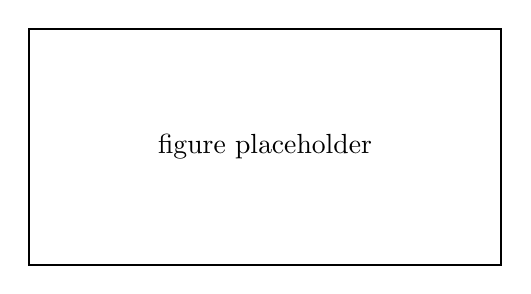
\begin{tikzpicture}
    \draw[thick] (0,0) rectangle (6,3);
    \node at (3,1.5) {figure placeholder};
  \end{tikzpicture}
  \caption{Example figure\label{fig:example}}
\end{figure}

% ---- Dropping in externally generated assets (R / Stata / Python) ----------
% \input a booktabs .tex for tables and a pgfplots/TikZ .tex (or
% \includegraphics a PDF) for figures:
%
% \input{table_regression.tex}
% \includegraphics[width=\textwidth]{figure_histogram.pdf}

\vspace{1\baselineskip}

{\RaggedRight \printbibliography}

\end{document}
